\documentclass{article}
\usepackage[utf8]{inputenc}
\usepackage[russian]{babel}
\usepackage{graphicx}
\usepackage{amsmath}
\usepackage{breqn}
\usepackage{wrapfig}
\usepackage{float}

\graphicspath{ {./data/images} }
\author{Александр Романов Б01-107}
\date{}
\title{3.6.1 Спектральный анализ электрических сигналов.}

\begin{document}
\maketitle
\section{Введение}
\subsection{Цель работы}
Изучить спектральный состав периодических электриче­
ских сигналов.
\subsection{В работе используются} 
Анализатор спектра, генератор прямоугольных импульсов и сигналов специальной формы,
осциллограф.

\subsection{Идеи}
\subsubsection{Разложение сложных сигналов в ряд Фурье}

При изучении линейных систем возникает необходимость представления произвольного
сигнла \(f(t)\) в виде ряда Фурье:
\[ f(t) = \sum_n c_ne^{i\omega_nt} \] 

Получим коэффициенты разложения в ряд Фурье для периодического колебательного процесса
общего вида \( f(t) = f(t + T) \), где \( T \) - период процесса. Покажем, что этом случае функция 
\( f(t) \) может быть представленна бесконечной суммой гармонических колебаний с кратными частотами:
\begin{equation} 
    f(t) = \sum_{n=-\infty}^{\infty} c_ne^{in\omega_0t}
    \label{sum_n}
\end{equation}

Нетрудно видеть, что все слогаемые в этой сумме -- периодические функции с периодом, кратным \(T\) и они
полностью исчерпывают набор гармонических функций, удовлетворяющих \( f(t) = f(t + T) \). Таким образом 
периодическая функция имеет дискретный спектр с кратными частотами.
Спектр -- то есть набор коэффициентов \(\{c_n\}\) -- можно найти следующим образом: домножим обе части
равенста (\ref{sum_n}) на \( e^{-im\omega_0t} \) и проинтегрируем по времени \(t\) за период (Например, от 0
до \(T\)). Получим

\begin{equation*}
    \int_0^T f(t)e^{-im\omega_0t}dt  \sum_n c_n \int_0^T e^{i(n - m)\omega_0t}dt
\end{equation*}

Вычислим интеграл в правой части:

\begin{equation*}
    \int_0^T e^{i(n-m)\omega_0t}dt = 
    \begin{cases}
        0 \quad if \: n \neq m\\
        T \quad if \: n = m\\
    \end{cases}
\end{equation*}

Таким образом получаем

\begin{equation}
    c_n = \frac{1}{T}\int_0^T f(t)e^{-in\omega_0t}dt.
    \label{eq_cn}
\end{equation}

\subsubsection{Периодическая последовательность прямоугольных импульсов}


\begin{figure}[H]
\centering
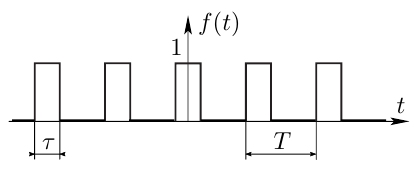
\includegraphics[width=0.5\textwidth]{sq_imp_example.png}
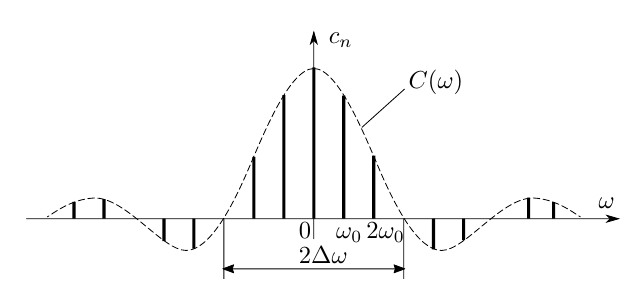
\includegraphics[width=0.5\textwidth]{sq_imp_spect_example.png}
\caption{Периодическая последовательность прямоугольных импульсов и её спектр(Для $\tau = \frac{T}{3}$).} 
\label{sq_imp_example}
\end{figure}
Рассмотрим сигнал на рис \ref{sq_imp_example} и найдём его спектр.
Используя (\ref{eq_cn}) на интегрвале интегрирования \( -T/2 \le t \le T/2 \), с учётом того, что функция 
\(f(t)\) отлична от нуля только лишь в области \( |t| < \tau/2 \) находим

\begin{equation}
    c_n = \frac{1}{T} \int_{-\tau/2}^{\tau/2} e^{-in\omega_0t}dt = \frac{\tau}{T} \cdot 
    \frac{\sin (n\omega_0\tau/2)}{n\omega_0\tau/2} = \frac{\sin (\pi n\tau/T)}{\pi n}
    \label{ep_cn_sq_imp}
\end{equation}

Пунктиром изображена огибающая кривая
\begin{equation*}
    C(\omega) = \frac{\tau}{T} \cdot \frac{\sin \omega \tau/2}{\omega\tau/2}
\end{equation*}

Полуширина \( \Delta \omega \) главного максимума этой функции определяется условием \( \sin \omega\tau/2 = 0 \):
\begin{equation*}
    \Delta\omega\cdot\tau = 2\pi
\end{equation*}




\subsubsection{Периодическая последовательность цугов гармонических колебаний}

\begin{figure}[H]
    \centering
    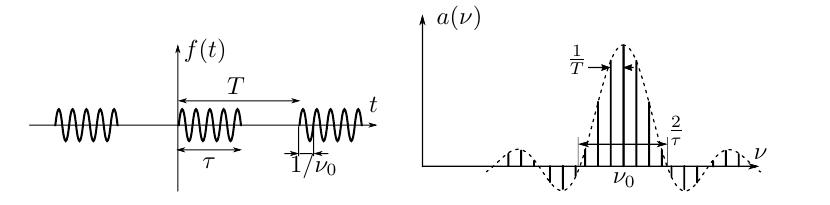
\includegraphics[width=\textwidth]{cug_imp_example.png}
    \caption{Периодическая последовательность синусоидальных цугов и её спектр. (Здесь \(T/\tau = 4\))} 
    \label{pic_cug_imp_example}
\end{figure}

Рассмотрим сигнал на рис \ref{pic_cug_imp_example}. Это - цуги колебания \( V_0\sin\omega_0t \).
Из (\ref{eq_cn}) найдём \(c_n\) и для них:

\begin{multline}
    c_n = \frac{2}{T}\int_{-\tau/2}^{\tau/2} V_0\cos(\omega_0t) \cdot \cos(n\Omega_1t)dt = \\
    = V_0 \frac{\tau}{T}\left(\frac{\sin\left[(\omega_0 - n\Omega_1)\frac{\tau}{2}\right]}
    {(\omega_0 - n\Omega_1)\frac{\tau}{2}} + \frac{\sin\left[(\omega_0 + n\Omega_1)\frac{\tau}{2}\right]}
    {(\omega_0 + n\Omega_1)\frac{\tau}{2}} \right)
    \label{eq_cn_cug}
\end{multline}

Тогда Спектры последовательности идентичны прямоугольным импульсам, но
сдвинуты на $\omega_0$.

\subsubsection{Амплитудно-модулированные колебания}
\begin{figure}[H]
    \centering
    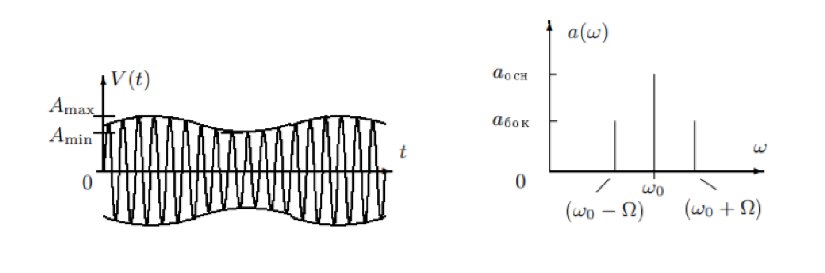
\includegraphics[width=\textwidth]{AM_signal_example.png}
    \caption{Амплитудно-модулированный сигнал и его спектр.} 
    \label{pic_am_sig_example}
\end{figure}

Рассмотрим рис. \ref{pic_am_sig_example} гармонические колебания высокой частоты $\omega_0$, амплитуда которых
медленно меняется по гармоническому закону с частотой $\Omega \ll \omega$.

\[ s(t) = A_0\left[1 + m \cos \Omega t\right] \cos \omega_0 t \]

Коэффициент $m$ называется \emph{глубиной модуляции}. При \( m < 1 \) амплитуда меняется от минимальной 
\( A_{min} = A_0(1 - m) \) до максимальной \( A_{max} = A_0(1 + m) \). Глубина модуляции может быть представленна
в виде

\[ m = \frac{A_{max} - A{min}}{A_{max} + A_{min}}. \]
Легко переписать уравнение сигнала как:

\begin{equation}
    f(t) = A_0 \cos \omega_0t + \frac{A_0m}{2} \cos \left(\omega_0 + \Omega\right)t  + \frac{A_0m}{2} 
    \cos \left(\omega_0 + \Omega\right)t.
    \label{eq_sig_am}
\end{equation}

Спектр таких колебаний содержит 3 составляющие. Основная компонента представляет собой исходное немодулированное
с несущей частотой \(\omega_0\) и амплитудой \(A_{cen} = A_0\) -- первое слагаемое в (\ref{eq_sig_am}); Боковые компоненты
спектра  соответствуют гармоническим колебания с частотами \((\omega_0 + \Omega)\) и \((\omega_0 - \Omega)\) -- второе
и третье слагаемые (\ref{eq_sig_am}). Амплитуды этих колебаний одинаковы и составляют \(m/2\) от амплитуды
немодулированного колебания \( A_{side} = A_0m/2\)


\subsubsection{Соотношения неопределённости}
\begin{figure}[H]
    \centering
    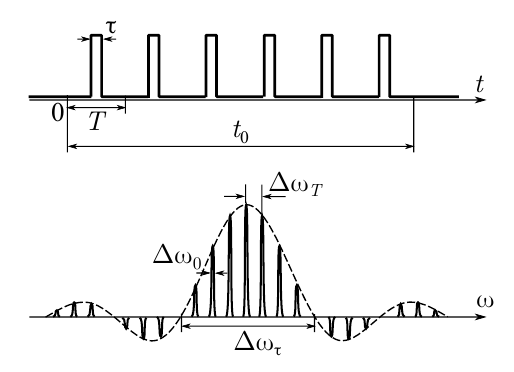
\includegraphics[width=0.8\textwidth]{uncertainty.png}
    \caption{Связь характерных масштабов спектра с характерными временами сигнала.} 
    \label{pic_uncertainty}
\end{figure}
При рассмотрении примеров мы получили соотношение, связы­вающее между собой длительность \(\Delta t\)сигнала с шириной
\(\Delta\omega\) его спектра:

\begin{equation}
    \Delta\omega\cdot\Delta t \sim 2\pi
    \label{uncertainty}
\end{equation}

Оказывается, это соотношение имеет весьма универсальный харак­тер. Оно остаётся справедливым
по порядку величины для произволь­ного сигнала \(f(t)\). Например, рассмотрим ограниченную последовательность
периодических импульсов с полной длительностью \(t_0\),  периодом \(T \ll t0\) и длительностью каждого импульса
\(\tau \ll T\). Сигнал и его спектр пред­ставлены на рис. \ref{pic_uncertainty} На спектре видно три характерных
масштаба частоты: масштаб \(\Delta\omega\tau = 2\pi/\tau\) -- это характерная ширина спектра, масштаб \(\Delta\omega T = 
2\pi\tau\) -- расстояние между соседними спектральными пиками, и наконец наименьший мас­штаб частоты, соответствующий
наибольшему характерному времени \(t_0\),определяет ширину каждого пика \(\Delta\omega_0 = 2\pi/t_0\).




\section{Работа}

\subsection{A. Исследование спектра периодической последовательности прямоугольных импульсов}

Устанавливаем на генераторе прямоугольные импульсы с \( \nu_{rep} = 1kHz \) и длительностью импульса
\( \tau = 100uS \). Получаем на экране спектр сигнала и, изменяя поочереди $\tau$ и $\nu_{rep}$ будем
наблюдать как изменяется спектр.

\begin{figure}[H]
    \centering
    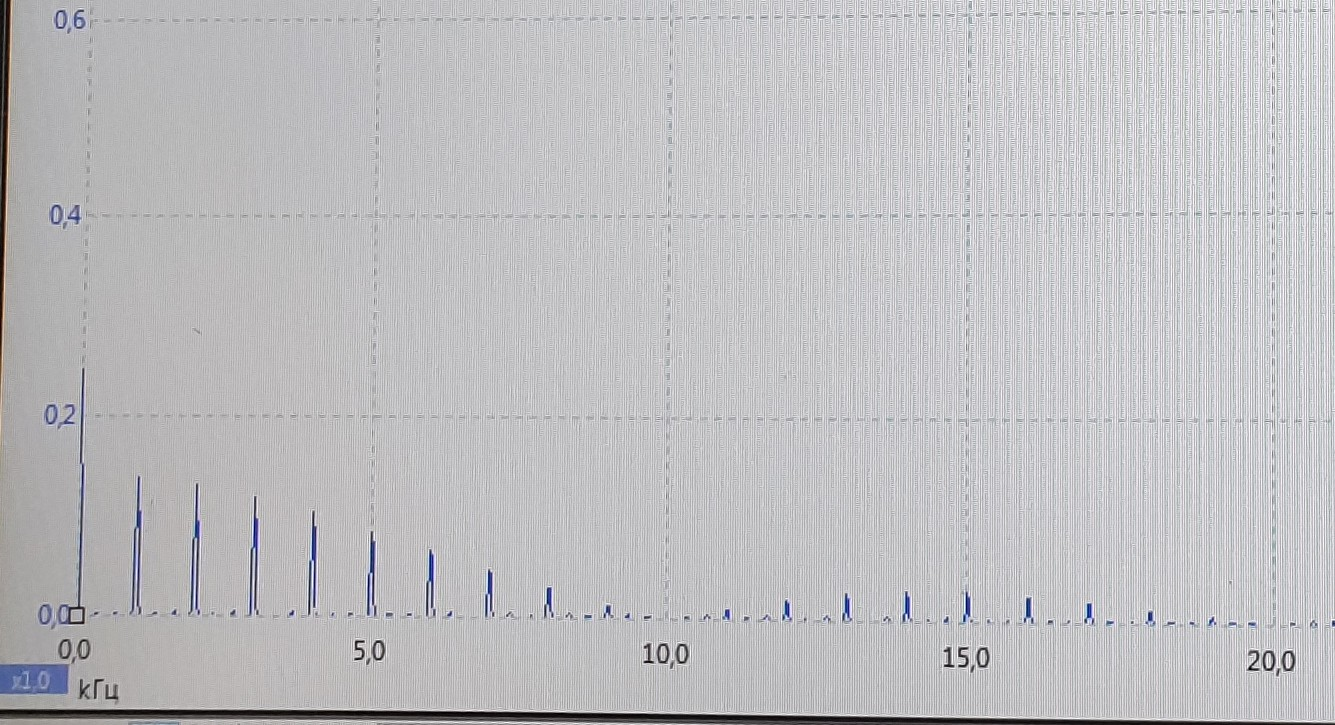
\includegraphics[width=0.6\textwidth]{1.jpg}
    \caption{Спектр при \( \nu_{rep} = 1 kHz, \tau = 100uS \)}
    \label{spec_1}
\end{figure}

\begin{figure}[H]
    \centering
    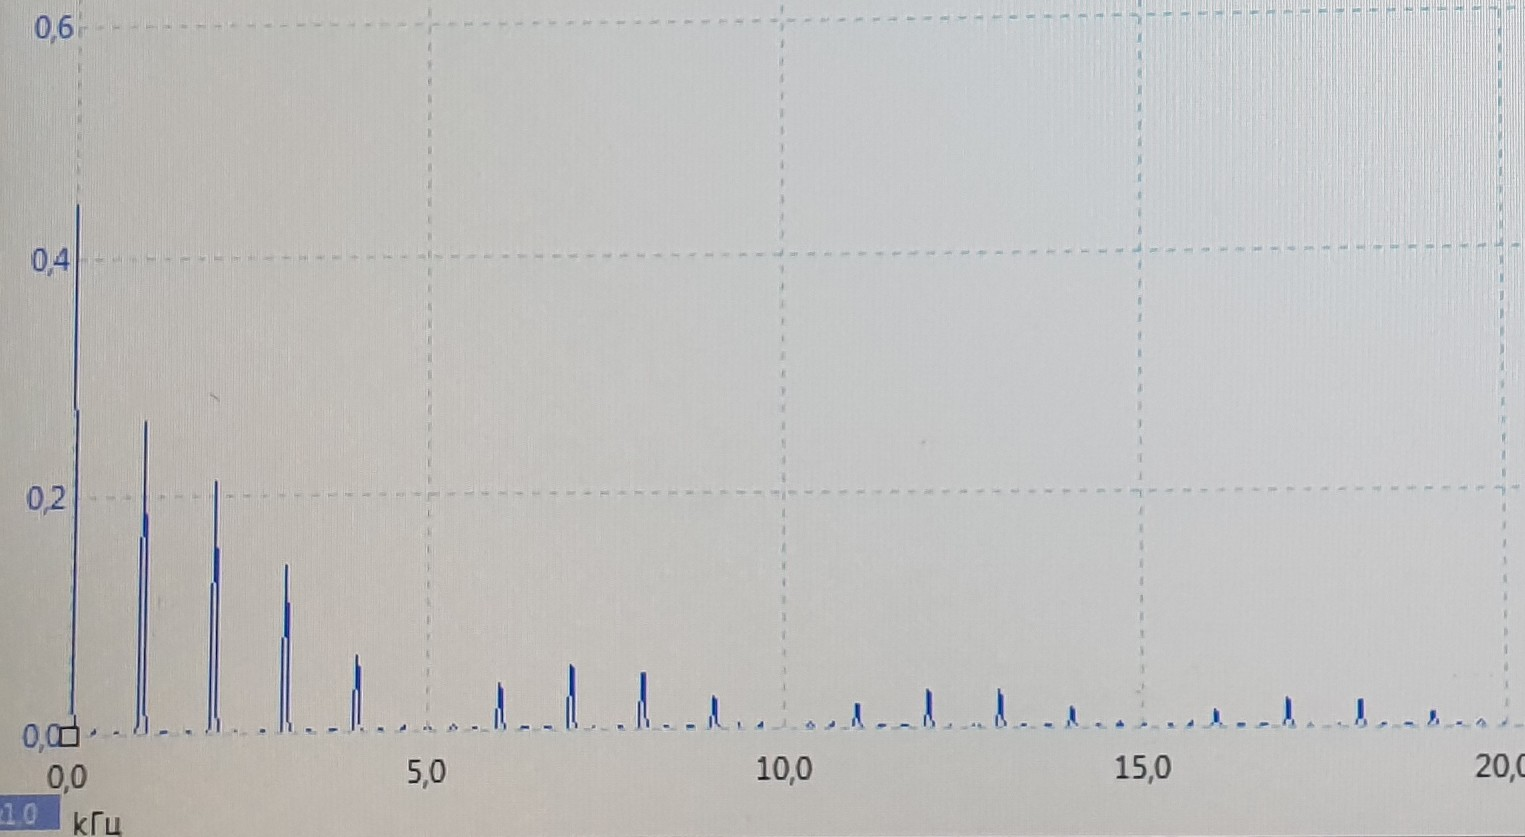
\includegraphics[width=0.6\textwidth]{2.jpg}
    \caption{Спектр при \( \nu_{rep} = 1 kHz, \tau = 200uS \)} 
    \label{spec_2}
\end{figure}

\begin{figure}[H]
    \centering
    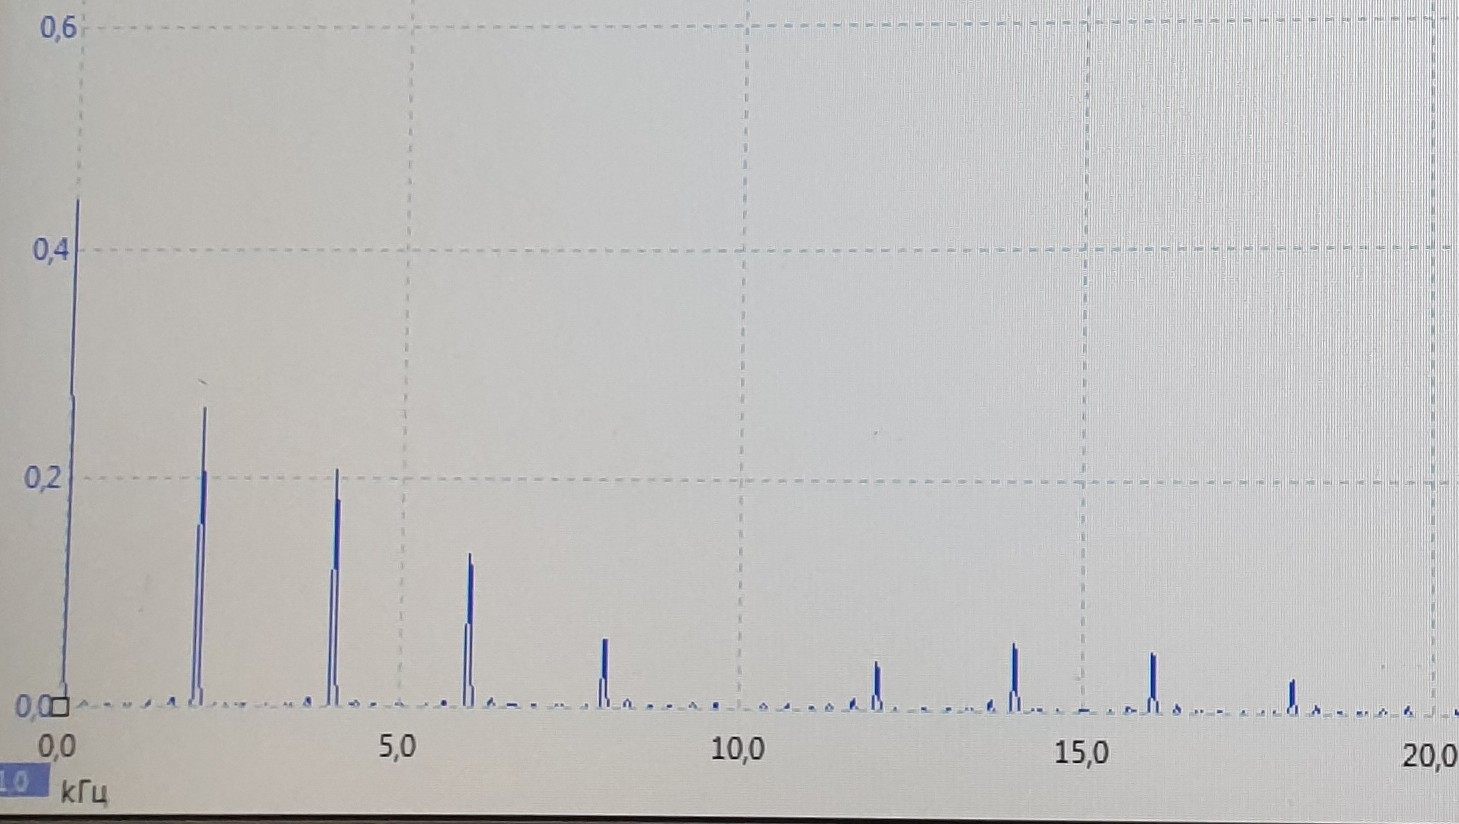
\includegraphics[width=0.6\textwidth]{3.jpg}
    \caption{Спектр при \( \nu_{rep} = 2 kHz, \tau = 100uS \)} 
    \label{spec_3}
\end{figure}

Проведём изерения зависимости ширины спектра от длительности импульса при частоте повторения \( \nu_{rep} = 1kHz \)

\begin{table}[H]
    \centering
    \label{tab_dnu_tau}
    \begin{tabular}{|c|c|}
        \hline
        \(\tau\), uS & \(\Delta\nu\), kHz \\\hline
        40                        & 25                  \\\hline
        60                        & 16                  \\\hline
        80                        & 13                  \\\hline
        100                       & 10                  \\\hline
        120                       & 8                   \\\hline
        140                       & 7                   \\\hline
        160                       & 6                   \\\hline
        180                       & 5.5                \\\hline
        200                       & 5                   \\\hline
    \end{tabular}
\end{table}

Получим отсюда таблицу \( \Delta\nu(1/\tau) \):


\begin{table}[H]
    \centering
    \label{tab_dnu_tau}
    \begin{tabular}{|c|c|}
        \hline
        \(1/\tau\), kHz & \(\Delta\nu\), kHz \\\hline
        25    & 25   \\\hline
        16.67 & 16   \\\hline
        12.5  & 13   \\\hline
        10    & 10   \\\hline
        8.33  & 8    \\\hline
        7.14  & 7    \\\hline
        6.25  & 6    \\\hline
        5.56  & 5.50 \\\hline
        5     & 5   \\\hline
    \end{tabular}
\end{table}

Построим график получившейся зависимости:
\begin{figure}[H]
    \centering
    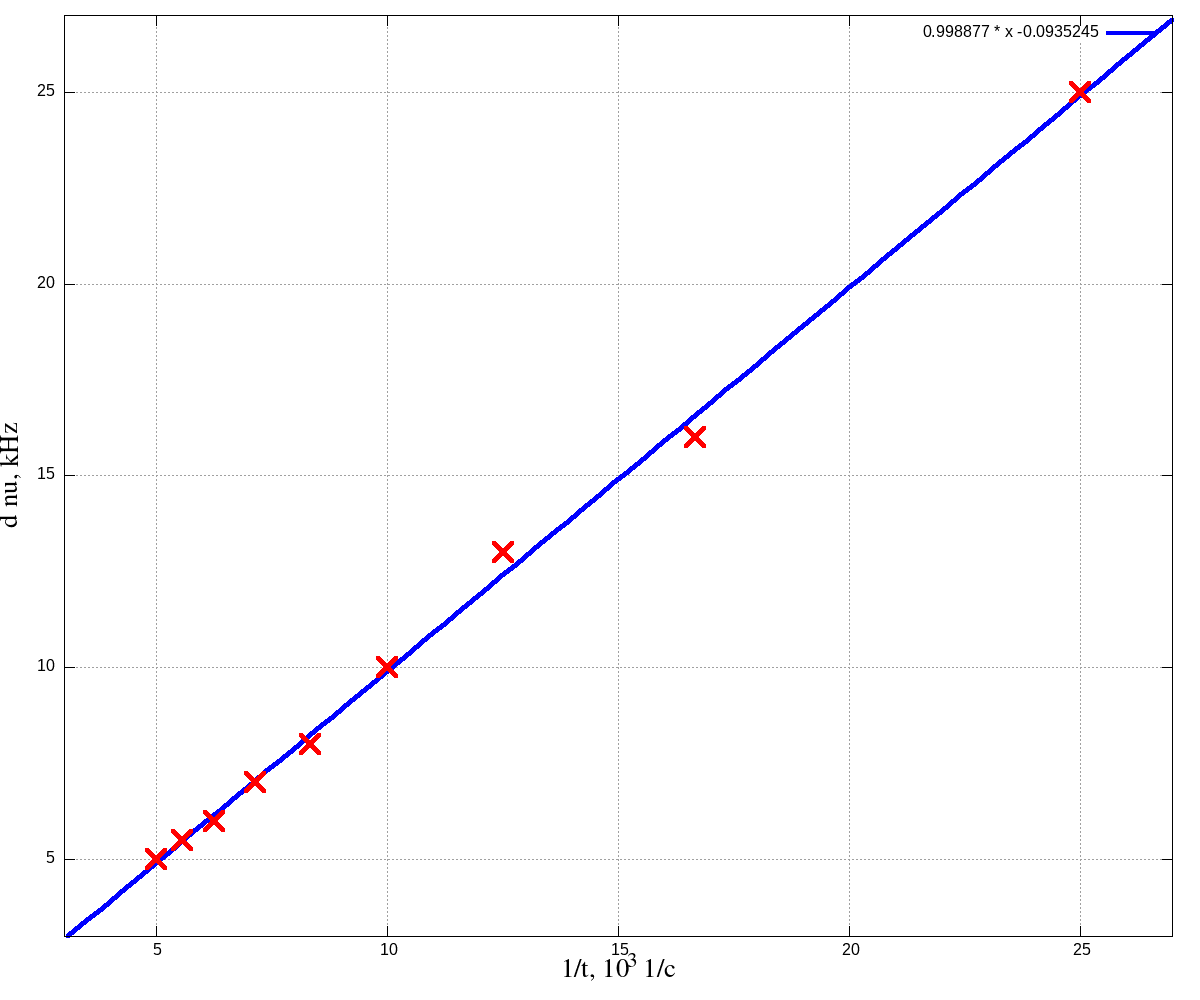
\includegraphics[width=0.8\textwidth]{dnu_tau.png}
    \caption{График \( \Delta\nu(1/\tau) \) для прямоугольных импульсов с \( \nu_{rep} = 1kHz \)}
    \label{pic_dnu_tau}
\end{figure}
Зависимость:

    \[ \Delta\nu = k \cdot \frac{1}{\tau} + b \]
    \[ k = (0.998 \pm 0.016) \]
    \[ b = (0.094 \pm 0.098) kHz\]

Мы видим, что действительно выполняется соотношение определённости:
\[ \Delta\nu\cdot\tau \simeq 1 \]

\subsection{B. Исследование спктра периодической последовательности цугов гармонических колебаний}

Установим частоту несущей \( \nu_0 = 25kHz \) и получим на экране осциллографа устойчивую картину цугов.

Будем наблюдать, как изменяется вид спектра:

\begin{figure}[H]
    \centering
    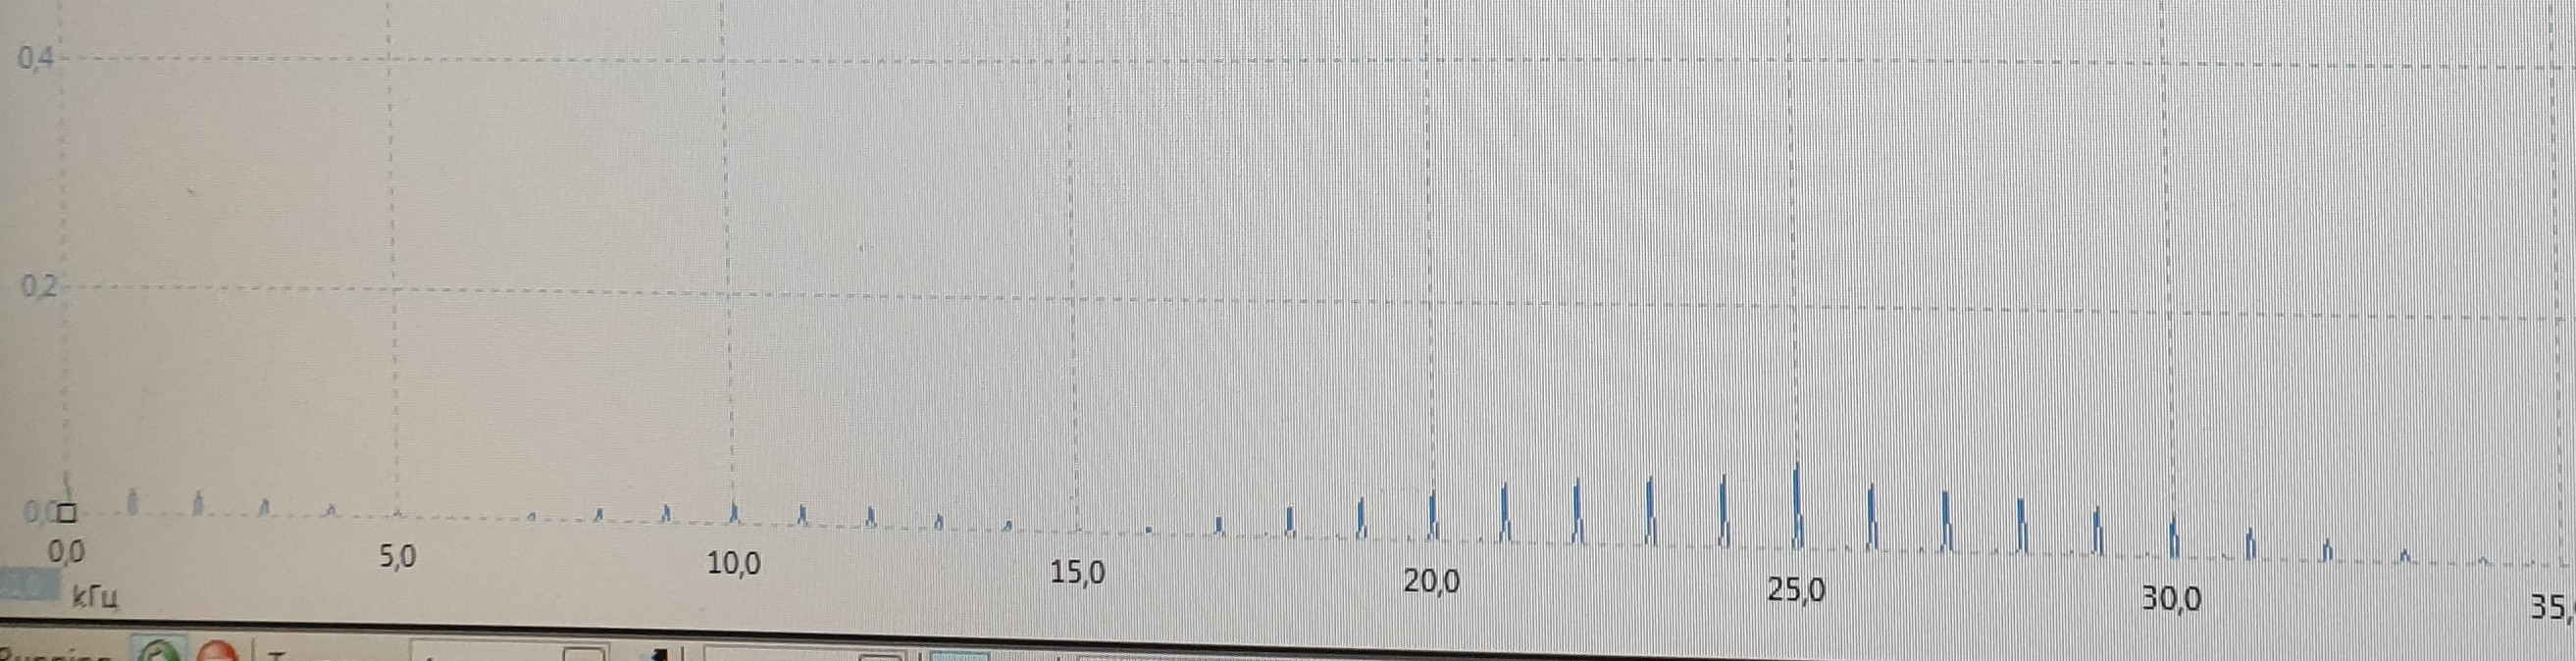
\includegraphics[width=0.6\textwidth]{cug_1.jpg}
    \caption{Спектр при \( \nu_{rep} = 1kHz, \nu_0 = 25 kHz, \tau = 100uS \)}
    \label{spec_cug_1}
\end{figure}

\begin{figure}[H]
    \centering
    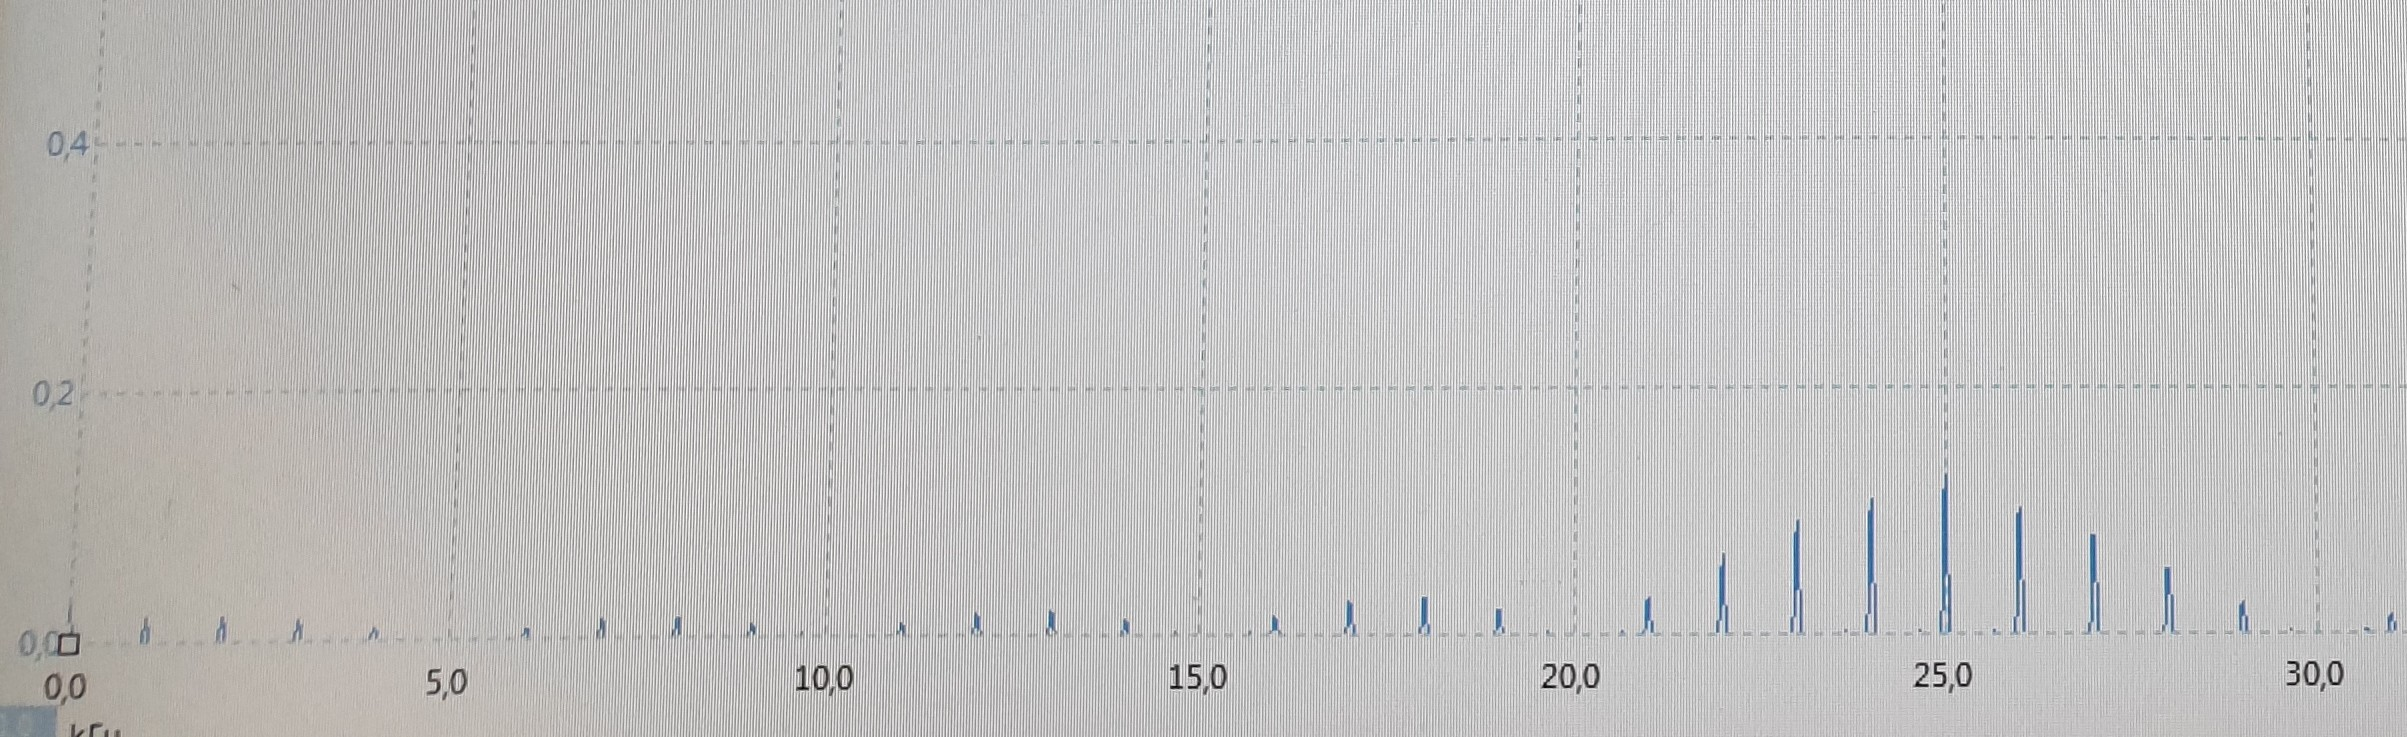
\includegraphics[width=0.6\textwidth]{cug_2.jpg}
    \caption{Спектр при \( \nu_{rep} = 1kHz, \nu_0 = 25 kHz, \tau = 200uS \)} 
    \label{spec_cug_2}
\end{figure}

\begin{figure}[H]
    \centering
    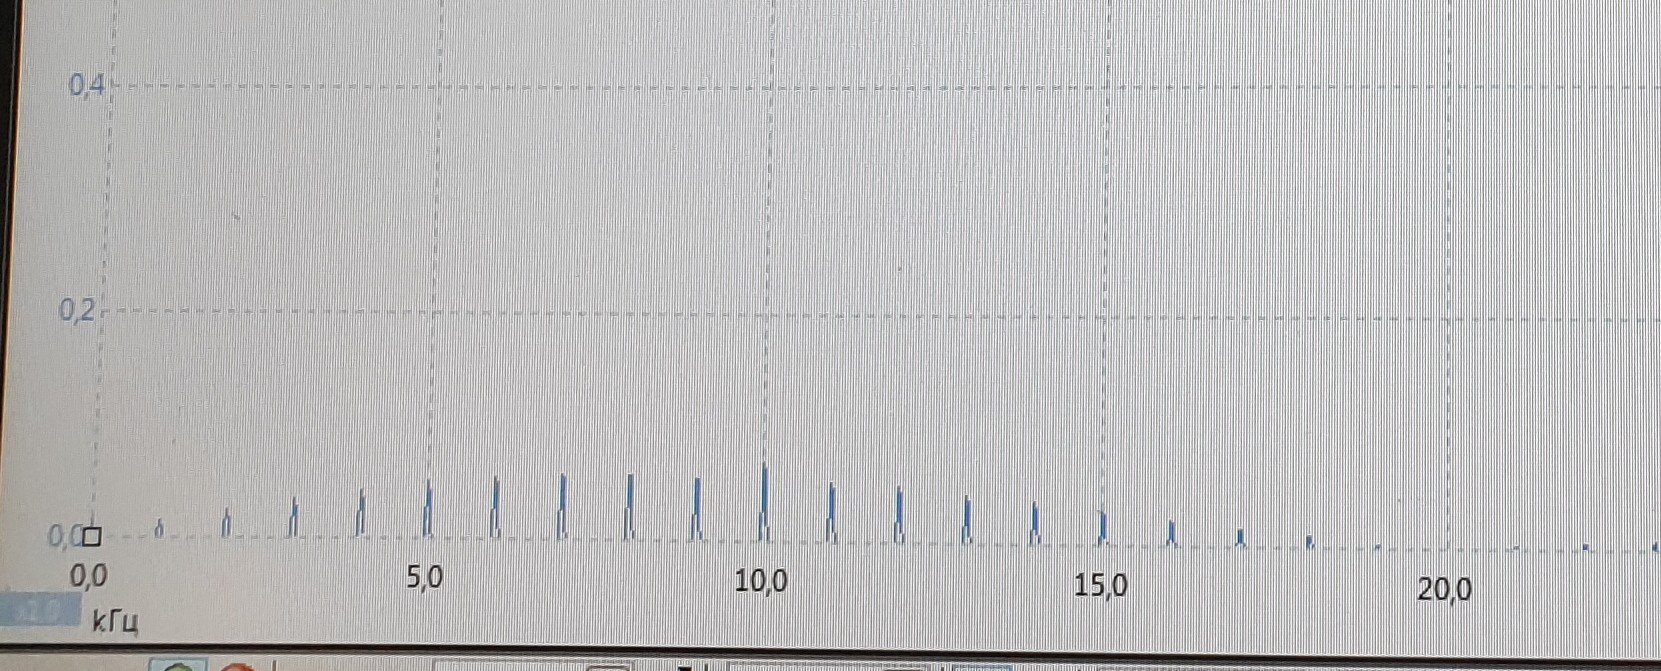
\includegraphics[width=0.6\textwidth]{cug_3.jpg}
    \caption{Спектр при \( \nu_{rep} = 1kHz, \nu_0 = 10 kHz, \tau = 100uS \)} 
    \label{spec_cug_2}
\end{figure}

\begin{figure}[H]
    \centering
    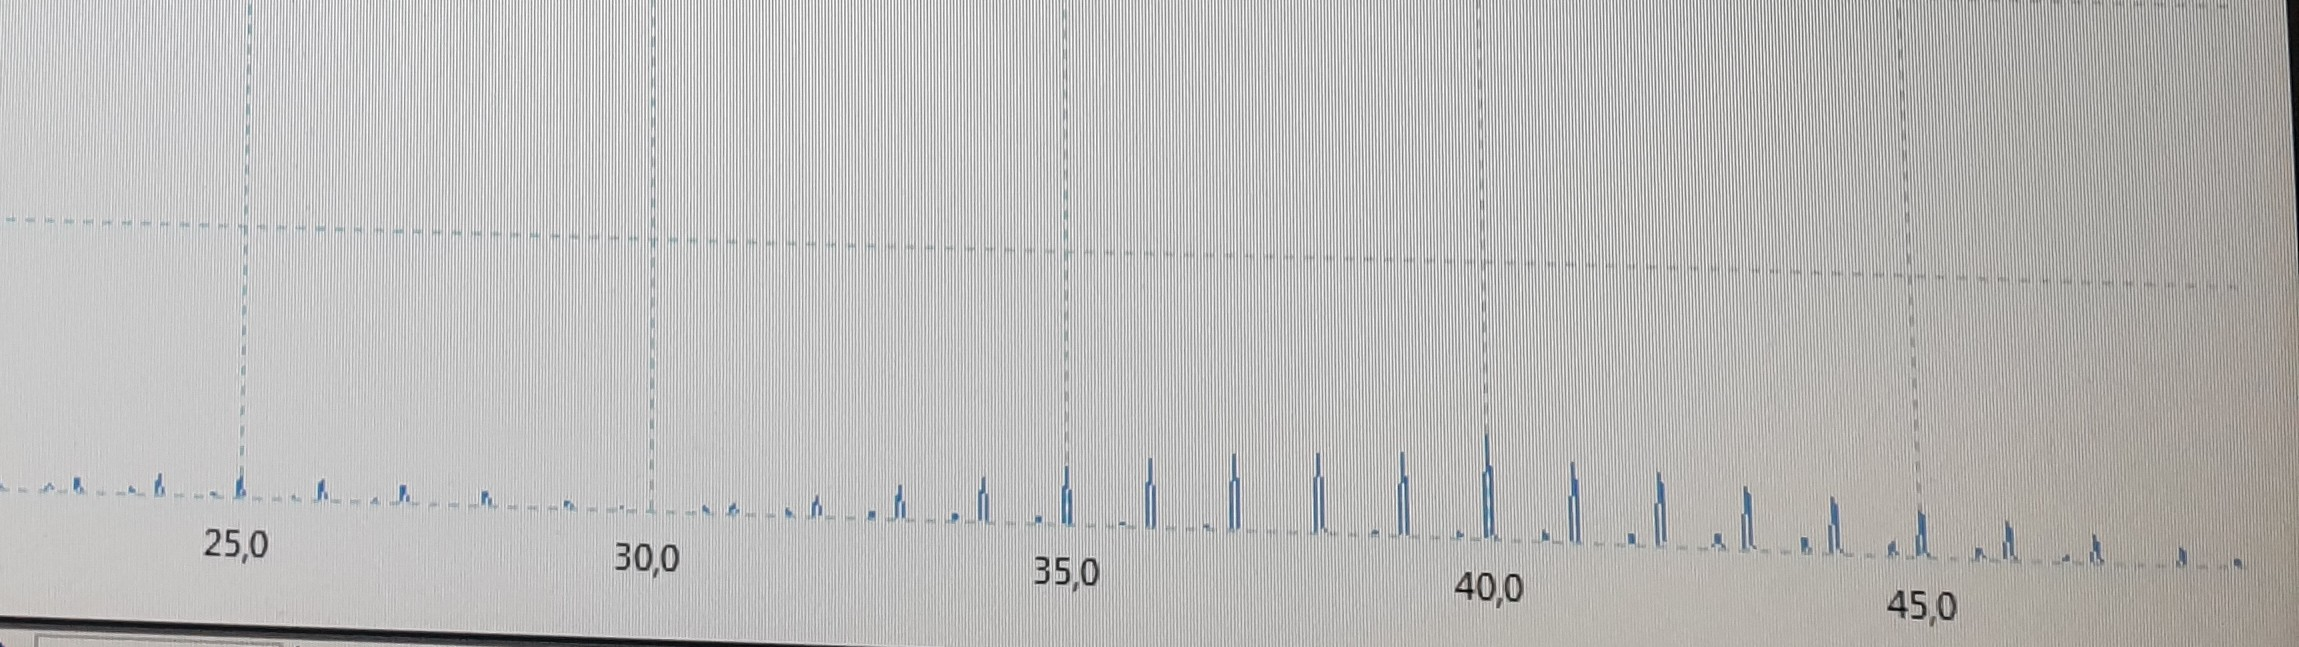
\includegraphics[width=0.6\textwidth]{cug_4.jpg}
    \caption{Спектр при \( \nu_{rep} = 1kHz, \nu_0 = 40 kHz, \tau = 100uS \)} 
    \label{spec_cug_2}
\end{figure}

\begin{figure}[H]
    \centering
    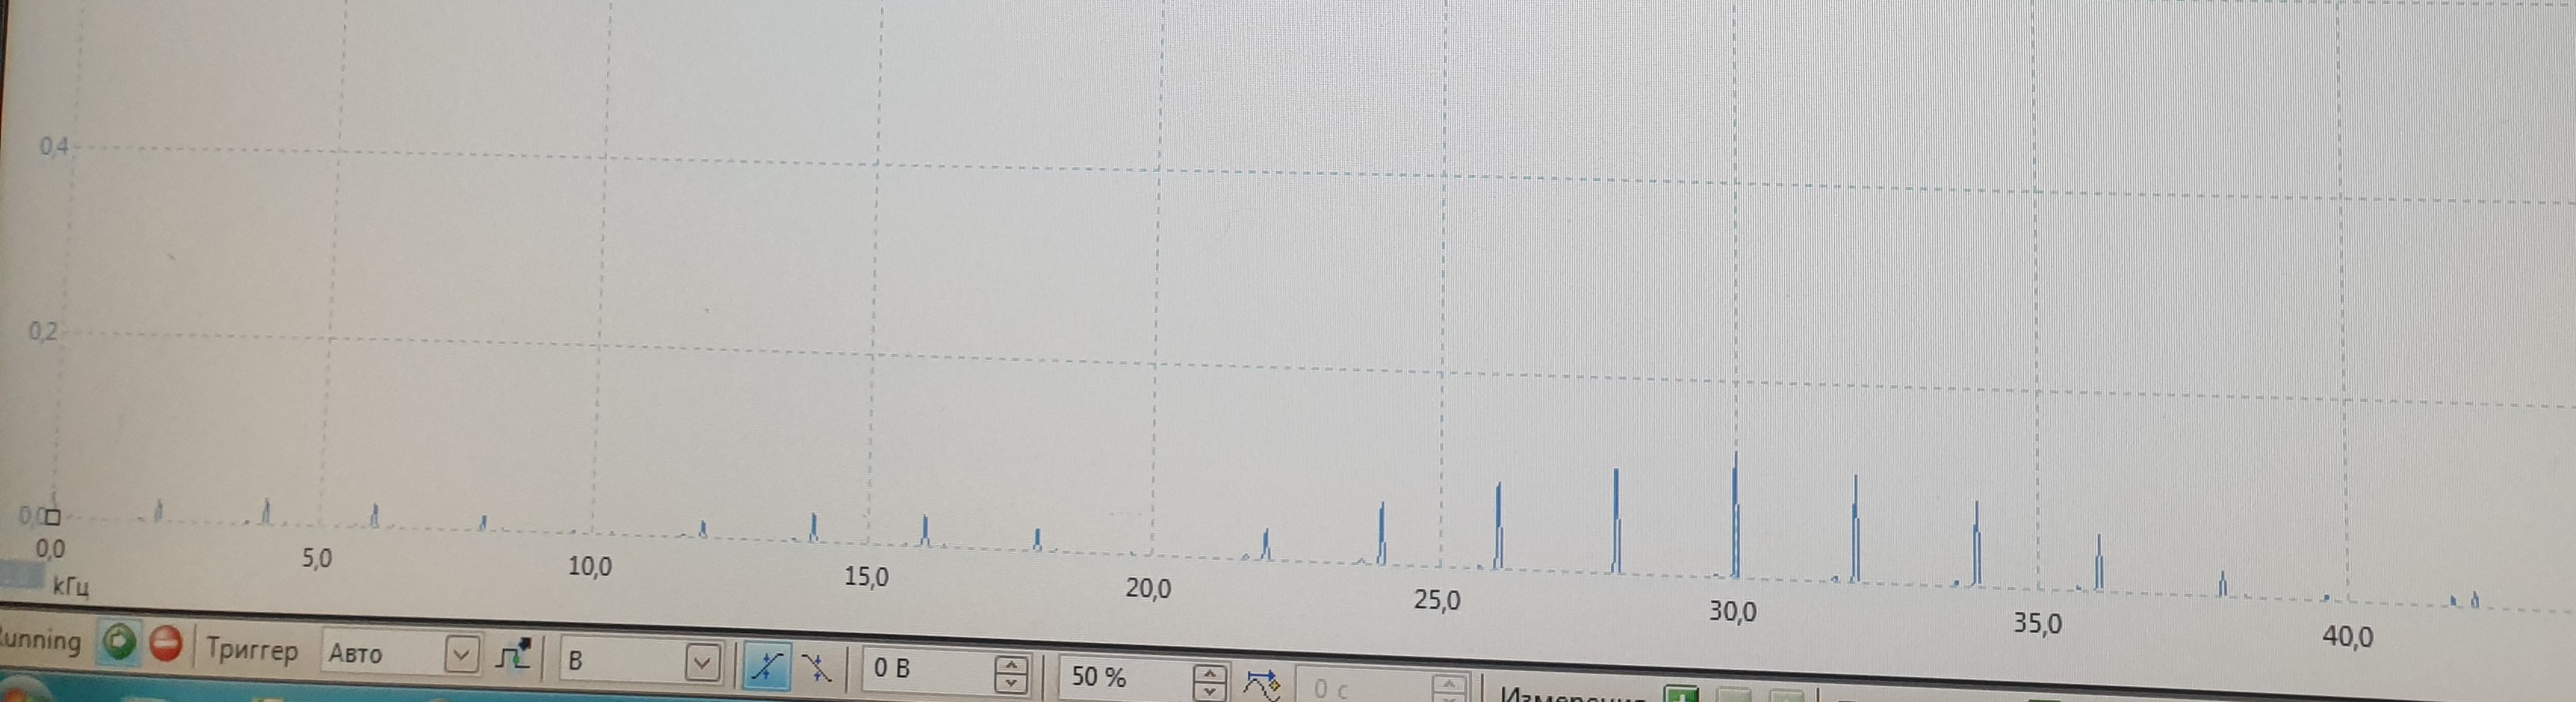
\includegraphics[width=0.6\textwidth]{cug_5.jpg}
    \caption{Спектр при \( \nu_{rep} = 2kHz, \nu_0 = 30 kHz, \tau = 100uS \)}
    \label{spec_cug_1}
\end{figure}

Исследуем зависимость \( \delta\nu (\nu_{rep}) \) при \( \tau = 100\) uS  и \(\nu_0 = 25\) kHz:


\begin{table}[H]
    \centering
    \begin{tabular}{|c|c|}
        \hline
        \(\delta\nu\), kHz & \(\nu_{rep}\), kHz\\\hline
        0.5 & 0.5 \\\hline
        1   & 1   \\\hline
        2   & 2   \\\hline
        4   & 4   \\\hline
        5   & 5   \\\hline
    \end{tabular}
\end{table}

\begin{figure}[H]
    \centering
    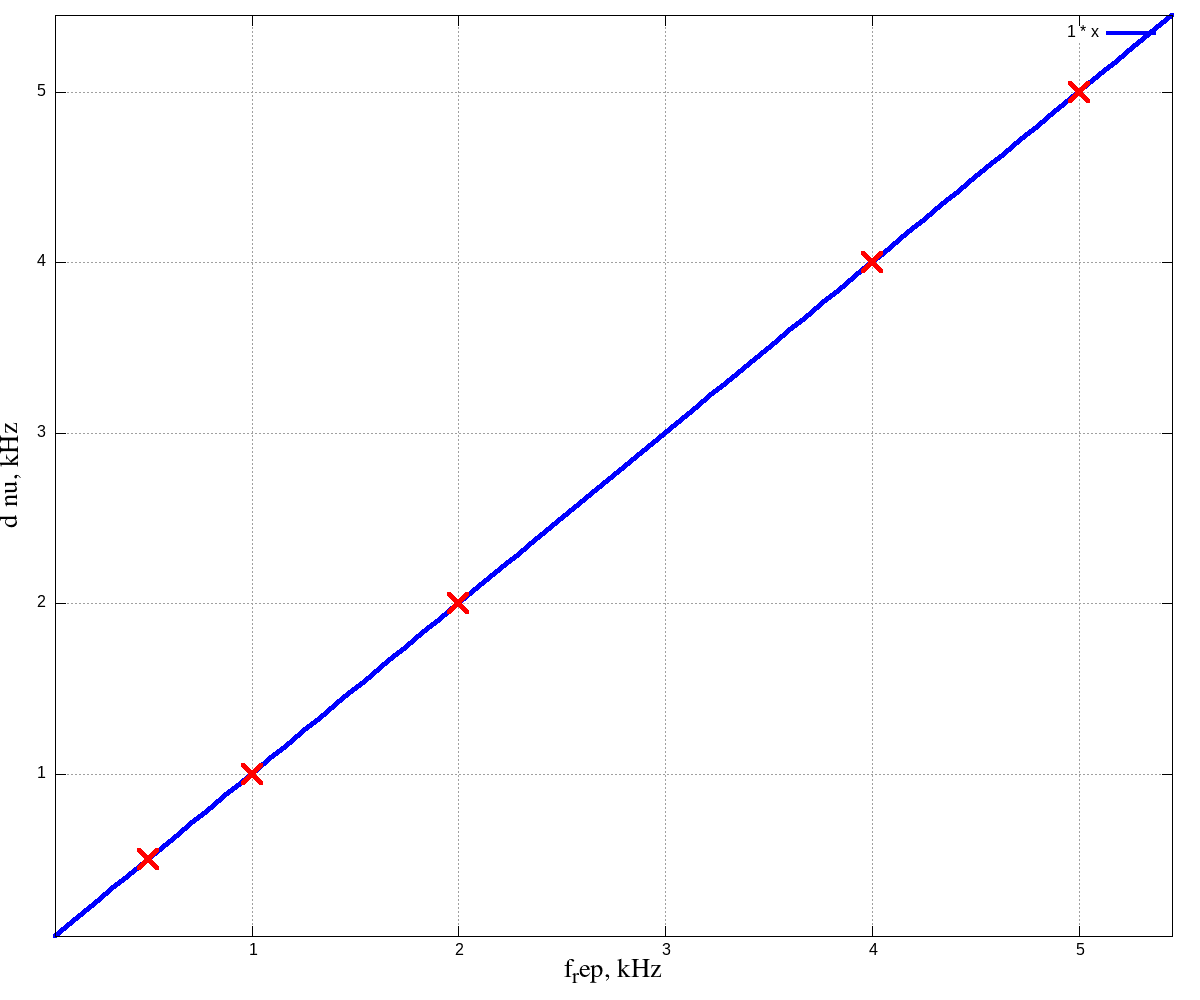
\includegraphics[width=0.8\textwidth]{dnu_frep.png}
    \caption{График \( \delta\nu(\nu_{rep}) \) для прямоугольных импульсов с \( \nu_0 = 25\) kHz и \(\tau = 100\) uS}
    \label{pic_dnu_tau}
\end{figure}

Завивисимость:

\[ \delta\nu = k\cdot\nu_{rep} + b \]
\[ k = (1.0 \pm 0.1) \]
\[ b = (0.0 \pm 0.1) kHz\]

Отсюда видно, что в данном случае тоже выполняется соотношение неопределённости
\[ \delta\nu\cdot T \simeq 1 \]


\subsection{C. Исследование спектра гармонических сигналов, модулированных по амплитуде}
Установим частоту несущей \( \nu_0 = 25 \) kHz, частоту модуляции \( \nu_{mod} = 1 \) kHz.
Получим спектр исследуемого сигнала. 
\begin{figure}[H]
    \centering
    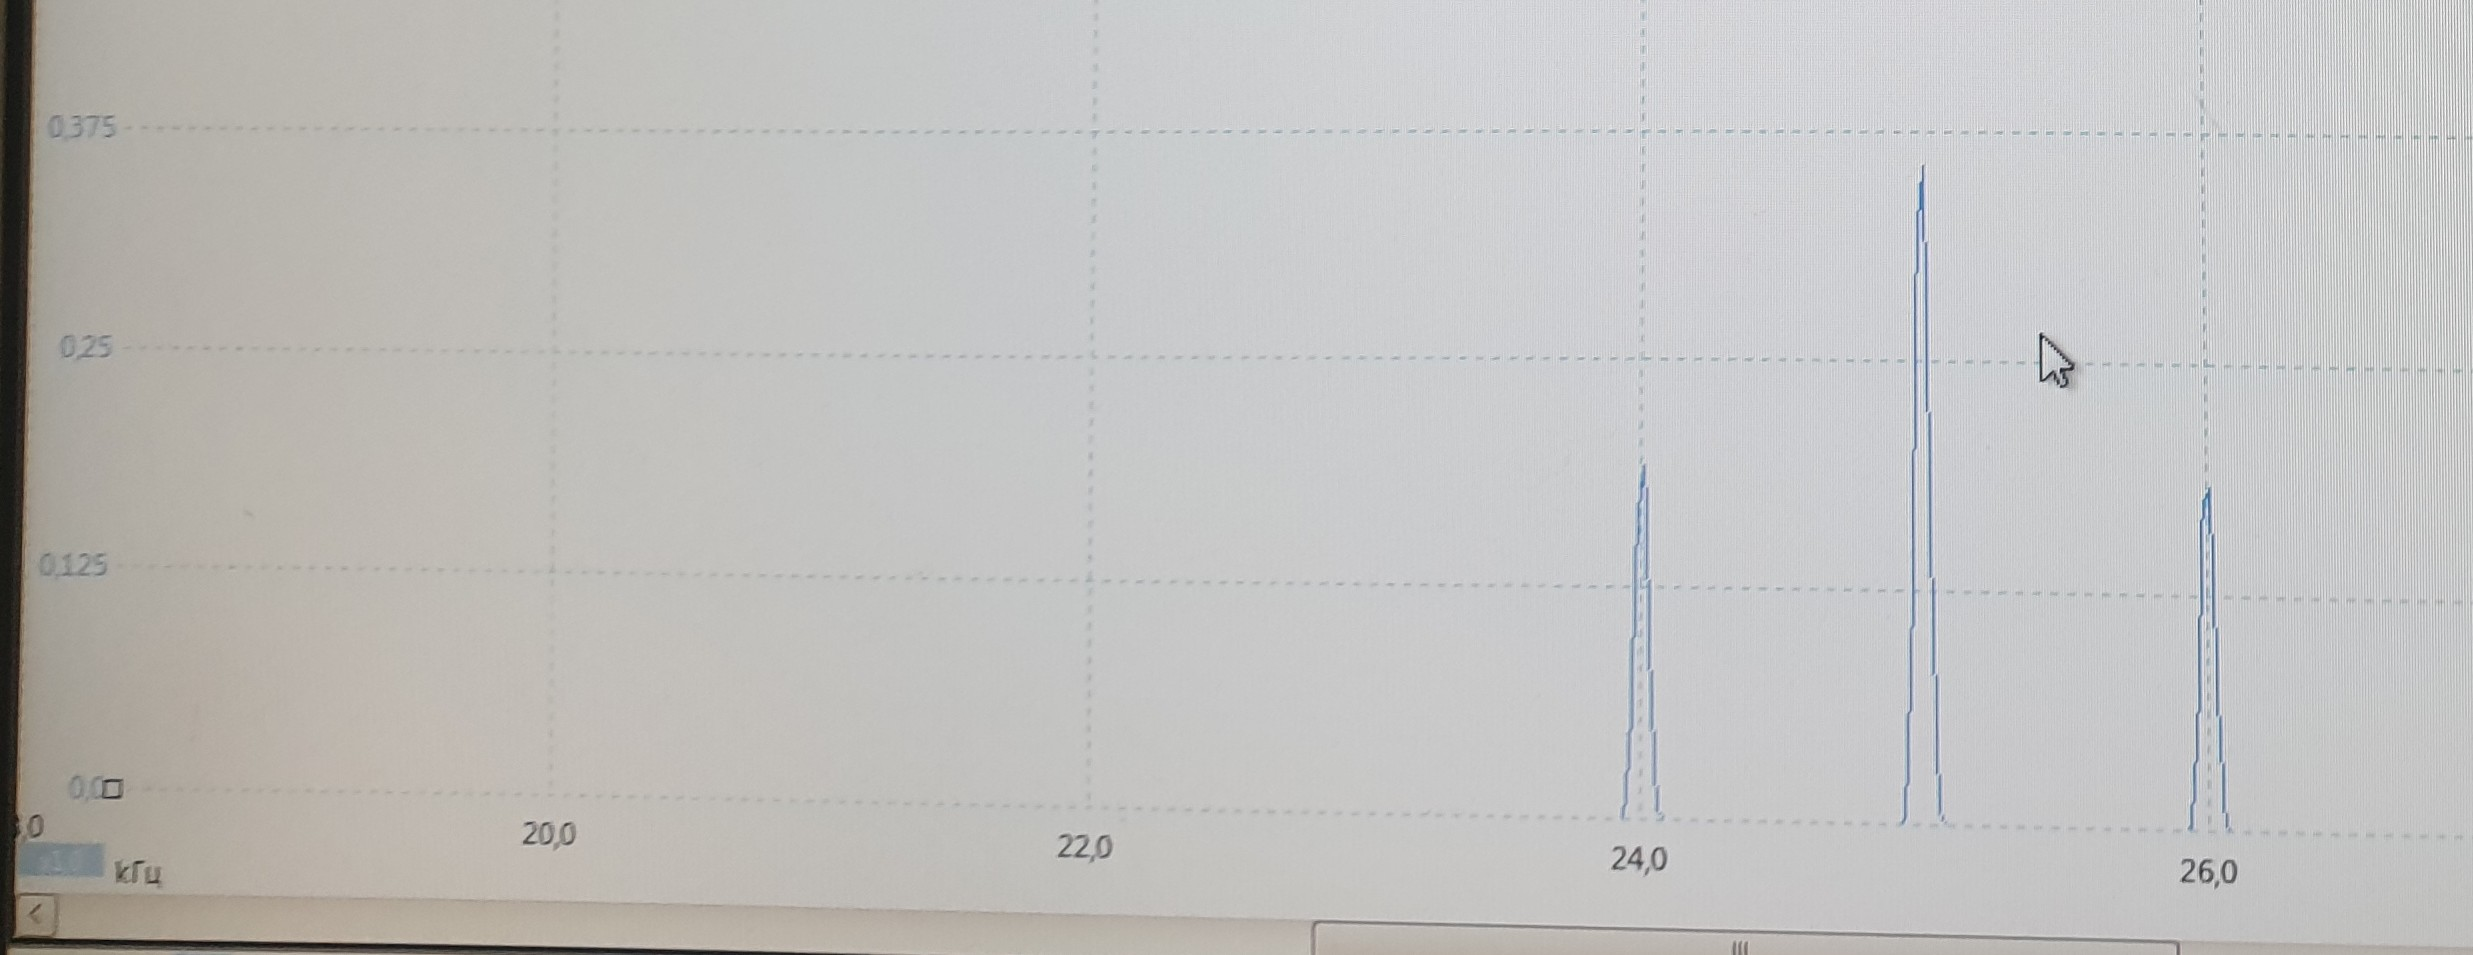
\includegraphics[width=0.8\textwidth]{mod_1.jpg}
    \caption{Спектр модулированного сигнала при \( m = 1 \).}
    \label{spec_mod}
\end{figure}

Будем изучать зависимость отношения амплитуд \( k = A_s/A_m \) боковой и основной частоты от 
параметра \(m = \left(A_{max} - A_{min}\right) / \left(A_{max} + A_{min}\right)\).


\begin{table}[H]
    \centering
    \begin{tabular}{|c|c|c|c|}
        \hline
        \(A_{m}\), mV &  \(A_{s}\), mV & \(m\) & \(k\) \\\hline
        322 & 16  & 0.1 & 0.050 \\\hline
        322 & 47  & 0.3 & 0.146 \\\hline
        322 & 75  & 0.5 & 0.233 \\\hline
        322 & 107 & 0.7 & 0.332 \\\hline
        322 & 139 & 0.9 & 0.431 \\\hline
        322 & 153 & 1.0 & 0.475 \\\hline
        \end{tabular}
\end{table}

\begin{figure}[H]
    \centering
    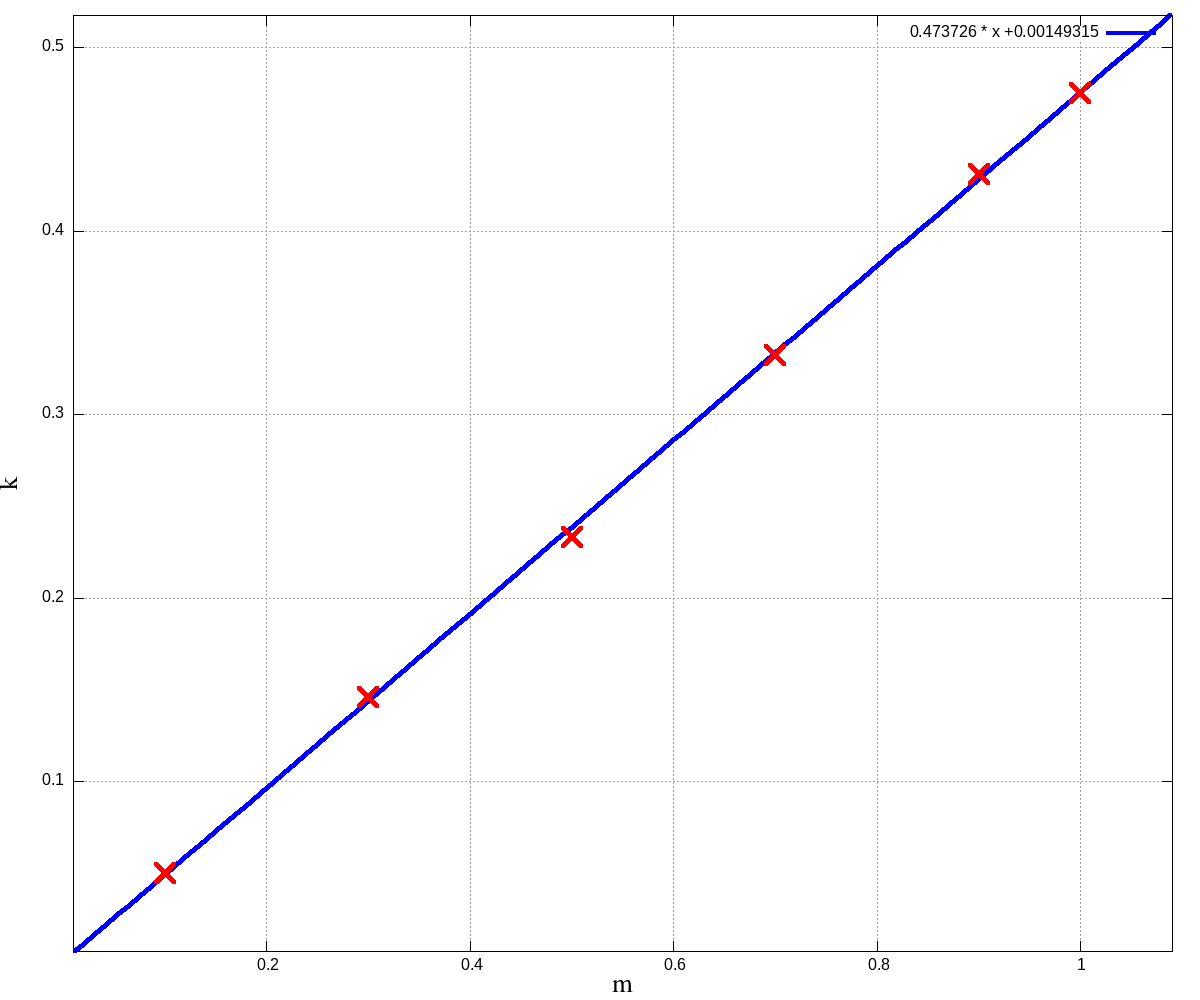
\includegraphics[width=0.8\textwidth]{mod.png}
    \caption{График \( k(m) \) для модулированного сигнала с \(\nu_0 = 25\) kHz, \(\nu_{mod} = 1\) kHz}
    \label{pic_dnu_tau}
\end{figure}

Полученная зависимость:

\[ k = a\cdot m + b \]
\[ a = (0.474 \pm 0.004) \]
\[ b = (0.001 \pm 0.001)\]

Получаем, что 
\[ \frac{k}{m} = 0.474 \pm 0.004 \]
Что сходится с теоретическим значением 0.5

\section{Выводы}

В этой работе

\begin{enumerate}
    \item Были изучены спектры и их зависимость от параметров для различных периодических
сигналов: Прямоугольных сигналов, гармонических цугов и амплитудно модулированного
гармонического сигнала.
    \item Были экспериментально проверены соотношения неопределённости
для различных видов сигналов.
    \item Была проверена справедливость разложения сигналов в ряд Фурье. Все сигналы и их спектры получились
именно такими, как показывали предварительные теоретические расчёты.
\end{enumerate}
\end{document}